% document LaTeX
\documentclass{book}
\usepackage{graphicx} % Pour insérer des images & figures
\usepackage[T1]{fontenc} % On lui dit qu'on veut encoder en T1 (encodage classique)
\usepackage[french]{babel} %On met les options entre crochets 
\usepackage{titlesec} % personnaliser le format des titres de section
\usepackage{hyperref} % Utilisé pour les liens hypertexte
\usepackage[toc]{glossaries} %glossaire
\usepackage{tocloft} % Charger le package tocloft
\usepackage[hmargin=2.5cm, vmargin=2cm]{geometry}
%gérer les marges
\usepackage{fancyhdr}
\usepackage{lipsum}
\usepackage{adjustbox}
\usepackage{hyperref}
\usepackage{enumitem}
\usepackage{float}
\usepackage{cleveref}
\usepackage{caption}
\usepackage[utf8]{inputenc}

\pagestyle{fancy}
\fancyhf{} % Efface tous les en-têtes et pieds de page actuels
\fancyhead[LE,RO]{\leftmark} % Nom du chapitre à gauche sur les pages impaires, à droite sur les pages paires
\fancyfoot[LE,RO]{\thepage} % Numéro de page à gauche sur les pages impaires, à droite sur les pages paires
%[C] = centre ; L = left ; LO = à gauche page impaires; LE = à gauche page paires ; R = droite
%\thepage = numéro de page
% tout ce qui commence par the = numéro du truc
%\fancyfoot[CO,CE]{Master}

%\renewcommand{\thechapter{\Roman{chapter}}}
%\usepackage{titlesec}
%\titleformat{\chapter}
%{\normalfont\Huge\bf}{\thechapter.}{20pt}
%{\chapfnt}

%\title{Rapport}
%\author{}

%\date{\today} %met la date du jour

% pour notre page de garde on a pas mal de restriction donc on va le faire différemment

%\makeatletter
%\renewcommand{\@chapapp}{}
%\makeatother %ces trois lignes permettent de ne pas afficher "chapitre 1" en haut à droite

% Redéfinition de la taille de la police pour la table des matières
\newcommand{\convertToBW}[1]{\adjustimage{filter=gray}{#1}}

\renewcommand{\cftchapfont}{\Large} % Reduire la taille de la police pour les chapitres
\renewcommand{\cftsecfont}{\large} % Reduire la taille de la police pour les sections
\renewcommand{\cftsubsecfont}{\normalsize} % Reduire la taille de la police pour les sous-sections

\DeclareUnicodeCharacter{FFFD}{\diamondquestionmark}

\begin{document}
%\maketitle on va faire une page vierge ou on va nous même tout insérer
%\large{texte à mettre en grand} %taille police
%\huge{texte}
%\large{texte}
%\small{texte}
%\tiny
%\scriptsize
%\footnotesize
%\thispagestyle{empty}

%%%%%%%%%%%%%%%%%%%%%%%%%%%%%%%%%%%%%%%%          1           %%%%%%%%%%%%%%%%%%%%%%%%%%%%%%%%%%%%%%%%%%%%%%%%%%%%%%%%%%%%%%%%%%%%%%%%%%%%%%%%%%%%%%%%%%%  Page de couverture   %%%%%%%%%%%%%%%%%%%%%%%%%%%%%%%%%%%%%%%%%%%%%
\newpage
\thispagestyle{empty}
%\vspace{1cm} %laisse un espace vertical de 1 cm
%\hspace{5cm} %espacer 2 images de 5cm
\vspace{-5cm}

\includegraphics[height=2cm]{univ.png}
\hfill

\includegraphics[height=1.5cm]{URN_NU_ST.jpg}

\vspace{0.5cm}
\hrule
\vspace{0.5cm}

\begin{center}
    \large{Université de Rouen Normandie - UFR Sciences et Techniques}
\end{center}

\begin{center}
    \large{Master 2 mention Bioinformatique – Parcours BIMS}
\end{center}

\begin{center}
    \large{2023 - 2024}
\end{center}

\vspace{1cm}

\begin{center}
    \Large{Rapport de stage}
\end{center}

\begin{center}
    \vspace{1cm}
    \hrule
    \vspace{1cm}
    \huge{Analyse textuelle d'article scientifiques evaluant l’impact des vers
        de terre sur l’environnement }
    \vspace{1cm}
    \hrule
    \vspace{1cm}
\end{center}

\begin{center}
    \large{Présenté et soutenu par}
\end{center}

\begin{center}
    \huge{Antoine Malet}
\end{center}

\begin{center}
    \vspace{1.5cm}
    \Large{Campus Agro Paris Saclay, Unité MIA Paris-Saclay} \\
    \Large{Equipe SOLsTIS}
\end{center}

\begin{center}
    \vspace{0.5cm}
    \large{Encadrants:} \\
    \vspace{0.5cm}
    \large{David Makowski} \\
    \large{Sophie Donnet}
\end{center}

\vspace{1.2cm}
\begin{center}
    
\includegraphics[height=2.3cm, width=15cm]{logos.png}
\end{center}

%%%%%%%%%%%%%%%%%%%%%%%%%%%%%%%%%%%%%%%%          2           %%%%%%%%%%%%%%%%%%%%%%%%%%%%%%%%%%%%%%%%%%%%%%%%%%%%%%%%%%%%%%%%%%%%%%%%%%%%%% Page vide pour le verso de la page de couverture%%%%%%%%%%%%%%%%%%%%%%%%%%%%%%%%%%%%%%%
\newpage
\thispagestyle{empty}
\mbox{} % Insère une boîte vide

%%%%%%%%%%%%%%%%%%%%%%%%%%%%%%%%%%%%%%%%          3           %%%%%%%%%%%%%%%%%%%%%%%%%%%%%%%%%%%%%%%%%%%%%%%%%%%%%%%%%%%%%%%%%%%%%%%%%%%%%%%%%%%%% Reprise de la page de couverture%%%%%%%%%%%%%%%%%%%%%%%%%%%%%%%%%%%%%%%%%%%%%%%%

\newpage
\thispagestyle{empty}
%\vspace{1cm} %laisse un espace vertical de 1 cm
%\hspace{5cm} %espacer 2 images de 5cm
\vspace{-5cm}

\includegraphics[height=2cm]{univBW.png}
\hfill

\includegraphics[height=1.5cm]{URN_NU_ST_BW.png}

\vspace{0.5cm}
\hrule
\vspace{0.5cm}

\begin{center}
    \large{Université de Rouen Normandie - UFR Sciences et Techniques}
\end{center}

\begin{center}
    \large{Master 2 mention Bioinformatique – Parcours BIMS}
\end{center}

\begin{center}
    \large{2023 - 2024}
\end{center}

\vspace{1cm}

\begin{center}
    \Large{Rapport de stage}
\end{center}

\begin{center}
    \vspace{1cm}
    \hrule
    \vspace{1cm}
    \huge{Analyse textuelle d'articles scientifiques evaluant l’impact des vers
        de terre sur l’environnement}
    \vspace{1cm}
    \hrule
    \vspace{1cm}
\end{center}

\begin{center}
    \large{Présenté et soutenu par}
\end{center}

\begin{center}
    \huge{Antoine Malet}
\end{center}

\begin{center}
    \vspace{1.5cm}
    \Large{Campus Agro Paris Saclay, Unité MIA Paris-Saclay} \\
    \Large{Equipe SOLsTIS}
\end{center}

\begin{center}
    \vspace{0.5cm}
    \large{Encadrant :} \\
    \vspace{0.5cm}
    \large{David Makowski} \\
    \large{Sophie Donnet}
\end{center}

\vspace{1.2cm}
\begin{center}
    
\includegraphics[height=2.3cm, width=15cm]{logosBW.png}
\end{center}

%%%%%%%%%%%%%%%%%%%%%%%%%%%%%%%%%%%%%%%%          3           %%%%%%%%%%%%%%%%%%%%%%%%%%%%%%%%%%%%%%%%%%%%%%%%%%%%%%%%%%%%%%%%%%%%%%%%%%%%%% Page vide pour le verso de la page de reprise %%%%%%%%%%%%%%%%%%%%%%%%%%%%%%%%%%%%%%%
%\newpage
%\thispagestyle{empty}
%\geometry{vmargin=2.5cm}
%\setlength\topmargin{0.2cm}

\newpage
\thispagestyle{empty}
\mbox{} % Insère une boîte vide

%%%%%%%%%%%%%%%%%%%%%%%%%%%%%%%%%%%%%%%%          4           %%%%%%%%%%%%%%%%%%%%%%%%%%%%%%%%%%%%%%%%%%%%%%%%%%%%%%%%%%%%%%%%%%%%%%%%%%%%%%%%%%%%%%%%%%%%%%%% Remerciements %%%%%%%%%%%%%%%%%%%%%%%%%%%%%%%%%%%%%%%%%%%%%%%%%%%%%

\newpage
\fancyhead[LE,RO]{REMERCIEMENTS}
% Début de la numérotation en chiffres romains
\pagenumbering{Roman}
\fancyfoot[C]{Antoine MALET - M1 Mention Bioinformatique Parcours BIMS - 2023-2024 - URN}
% Supprimer la ligne horizontale de l'en-tête pour cette page spécifique
%\thispagestyle{fancy} % Réappliquer le style fancy pour les autres pages
%\renewcommand{\headrulewidth}{0pt}   % Supprimer la ligne horizontale de l'en-tête

%\thispagestyle{plain} % Utiliser le style plain pour cette page spécifique (sans en-tête)

%  \begin{center}
%    \huge{\textbf{Remerciements}}
%\end{center}
%\vspace{1.5cm}

%\chapter*{Remerciements} l'étoile signifie que la section ne sera pas incluse dans la numérotation automatique des sections et ne sera pas ajoutée à la table des matières.
\chapter*{Remerciements}
\addcontentsline{toc}{chapter}{Remerciements}

\noindent
\large{En premier lieu, j'aimerais remercier mes encadrants pour ce stage, Mme Sophie DONNET et
    M. David MAKOWSKI, pour avoir accepté ma candidature et acceuilli au sein de
    leur équipe. Merci aussi pour leurs conseils et leurs effort d'accompagnement et de relecture de mes travaux! Je tiens aussi à adresser un mot particulier à mes vaillants collègues de bureau Emré ANAKOK et Caroline COGNOT, pour leur compagnie perpétuelle et leurs très bons
    conseils.}
\par % Nouveau paragraphe
Je remercie aussi Louis LACOSTE, pour ses excellents conseils en R et en cinématographie, ainsi que François VICTOR, pour ses généreuses explications en statistiques théoriques auxquelles je n'ai pas compris grand-chose. Merci aussi à Armand FAVROT, pour son acceuil et ses invitations aux Eventos des repas organisés par la cafet (les fraises maison étaient légendaires !). Enfin, chaleureuses salutations à tous mes collègues de pause café, qui sont toujours restés sympathiques et acceuillants même si je n'ai jamais bu la moindre goutte de café. Courage, peut-être qu'un jour vous me convertirez à votre religion!

Merci enfin à tous ceux que je n'ai pas nommés, particulièrement aux personnels qui prennent soin des locaux en silence, sans qui l'infrastructure de travail ne pourrait pas fonctionner correctement.

% Ne pas mettre le texte "Chapitre 1" de l'en-tête
\thispagestyle{fancy}
\clearpage % Aller à la page suivante

%%%%%%%%%%%%%%%%%%%%%%%%%%%%%%%%%%%%%%%%          5           %%%%%%%%%%%%%%%%%%%%%%%%%%%%%%%%%%%%%%%%%%%%%%%%%%%%%%%%%%%%%%%%%%%%%%%%%%%%%%%%%%%%%%%%%% Vide (verso remerciements) %%%%%%%%%%%%%%%%%%%%%%%%%%%%%%%%%%%%%%%%%%%%%%%%

\newpage
\mbox{} % Insère une boîte vide
\thispagestyle{fancy}

%%%%%%%%%%%%%%%%%%%%%%%%%%%%%%%%%%%%%%%%          6           %%%%%%%%%%%%%%%%%%%%%%%%%%%%%%%%%%%%%%%%%%%%%%%%%%%%%%%%%%%%%%%%%%%%%%%%%%%%%%%%%%%%%%%%%%%   Table des matières  %%%%%%%%%%%%%%%%%%%%%%%%%%%%%%%%%%%%%%%%%%%%%%%%

\newpage
\fancyhead[LE,RO]{\leftmark}
\tableofcontents %table des matieres , normalement il faut compiler 2 fois mais pas besoin sur overleaf
\addcontentsline{toc}{chapter}{Table des matières}
\thispagestyle{fancy}

%%%%%%%%%%%%%%%%%%%%%%%%%%%%%%%%%%%%%%%%          7           %%%%%%%%%%%%%%%%%%%%%%%%%%%%%%%%%%%%%%%%%%%%%%%%%%%%%%%%%%%%%%%%%%%%%%%%%%%%%%%%%%%%%%%%%% Vide (verso TOC) %%%%%%%%%%%%%%%%%%%%%%%%%%%%%%%%%%%%%%%%%%%%%%%%

\newpage
\mbox{} % Insère une boîte vide

%%%%%%%%%%%%%%%%%%%%%%%%%%%%%%%%%%%%%%%%          8           %%%%%%%%%%%%%%%%%%%%%%%%%%%%%%%%%%%%%%%%%%%%%%%%%%%%%%%%%%%%%%%%%%%%%%%%%%%%%%%%%%%%%%%%%% Table des illustrations %%%%%%%%%%%%%%%%%%%%%%%%%%%%%%%%%%%%%%%%%%%%%%%%

\newpage
\listoffigures %ajoute la table des figures
\thispagestyle{fancy}

%%%%%%%%%%%%%%%%%%%%%%%%%%%%%%%%%%%%%%%%          9           %%%%%%%%%%%%%%%%%%%%%%%%%%%%%%%%%%%%%%%%%%%%%%%%%%%%%%%%%%%%%%%%%%%%%%%%%%%%%%%%%%%%%%%%%% Vide (verso TOF) %%%%%%%%%%%%%%%%%%%%%%%%%%%%%%%%%%%%%%%%%%%%%%%%

\newpage
\mbox{} % Insère une boîte vide

%%%%%%%%%%%%%%%%%%%%%%%%%%%%%%%%%%%%%%%%          10          %%%%%%%%%%%%%%%%%%%%%%%%%%%%%%%%%%%%%%%%%%%%%%%%%%%%%%%%%%%%%%%%%%%%%%%%%%%%%%%%%%%%%%%%%% Liste des abréviations %%%%%%%%%%%%%%%%%%%%%%%%%%%%%%%%%%%%%%%%%%%%%%%%

\newpage
\fancyhead[LE,RO]{LISTE DES ABRÉVIATIONS}
\chapter*{Liste des Abréviations}
\addcontentsline{toc}{chapter}{Liste des Abréviations}

\begin{description}
    \item[ASCII] American Standard Code for Information Interchange
    \item[API] Application Programming Interface
    \item[CSS] Cascade Style Sheet
    \item[DOI] Digital Object Identifier
    \item[HTML] Hypertext Markup Language
    \item[IDE] De l'anglais, Environnement de Développement Intégré
    \item[MA] Métaanalyse
    \item[MIA] Mathématiques et Informatique Appliquée
    \item[Rmd] R Markdown
    \item[RG] ResearchGate
    \item[RGS2] ResearchGateScrapper2.py
    \item[UMR] Unité Mixte de Recherche

\end{description}
% REMOVE
\thispagestyle{fancy}

%%%%%%%%%%%%%%%%%%%%%%%%%%%%%%%%%%%%%%%%          11          %%%%%%%%%%%%%%%%%%%%%%%%%%%%%%%%%%%%%%%%%%%%%%%%%%%%%%%%%%%%%%%%%%%%%%%%%%%%%%%%%%%%%%%%%% Verso Liste des abréviations %%%%%%%%%%%%%%%%%%%%%%%%%%%%%%%%%%%%%%%%%%%%%%%%

\newpage
\mbox{} % Insère une boîte vide
\thispagestyle{fancy}

%%%%%%%%%%%%%%%%%%%%%%%%%%%%%%%%%%%%%%%%          12         %%%%%%%%%%%%%%%%%%%%%%%%%%%%%%%%%%%%%%%%%%%%%%%%%%%%%%%%%%%%%%%%%%%%%%%%%%%%%%%%%%%%%%%%%% Glossaire %%%%%%%%%%%%%%%%%%%%%%%%%%%%%%%%%%%%%%%%%%%%%%%%


\newpage
\fancyhead[LE,RO]{GLOSSAIRE}
\chapter*{Glossaire}


\begin{description}

    \item[JSON:] JSON (JavaScript Object Notation) est un format de fichier textuel conçu pour la structuration et l’échange de données (https://www.hostinger.fr/tutoriels/quest-ce-que-json).

    \item[Markdown:] Markdown est un langage de balisage léger qui permet de
        formater du texte de manière simple et rapide. Il utilise des caractères
        spéciaux pour indiquer les éléments de mise en forme, tels que les titres, les
        listes, les liens, etc. Les fichiers Markdown peuvent être convertis en HTML
        pour être affichés sur un site web ou dans un logiciel de traitement de texte
        (source: https://bility.fr/definition-markdown/).

    \item[Métaanalyse:] Article scientifique présentant la combinaison des résultats statistiques d'une série d'études indépendantes sur un problème donné. 

    \item[N-gram:] Suite de mots consécutifs de taille n (une des possibilités
        de tokenisation). Utile pour comprendre les relations logiques entre les mots. Les bigrammes sont un cas particulier de n-gram (n-gram de longueur 2).

    \item [Racinisation (linguistique):] Obtention du radical, par exemple par dépréfixation ou \sloppy désuffixation (\textit{Exemple:}"enhance", "enhances" et "enhancement" deviennent tous "enhanc").
    
    \item [Réseau de n-grams:] Figure permettant de visualiser toutes les relations entre les différents tokens simultanément, plutôt que deux par deux. Cela permet d'aller plus loin que l'analyse de bigrammes séparés les uns des autres.

    \item[Sélecteurs CSS:] Les sélecteurs définissent les éléments sur
        lesquelles s'applique un ensemble de règles CSS (langage de programmation employé pour mettre en forme une page Web). Ils peuvent être employés en
        Web scraping pour cibler et isoler certains éléments d'intérêt.

    \item[Token:] Unité textuelle souvent réduite, voire ne comprenant qu'un
        seul mot, issue du processus de tokenisation.

    \item[Tokenisation:] Processus consistant à découper un texte ou un corpus
        de textes en unités textuelles plus réduites, comme des mots, des n-grams ou
        des phrases.

    \item[Text-mining:] Processus d'analyse textuelle consistant à transformer
        un texte non structuré en données structurées pour ensuite procéder à
        l’analyse. Cette pratique repose sur la technologie de « Natural Language
        Processing » (traitement du langage naturel), permettant aux machines de
        comprendre et de traiter le langage humain automatiquement (source :
        https://datascientest.com/text-mining-definition).

    \item[Web scraping:] Technique permettant d’extraire automatiquement de
        grandes quantités d’informations d’un site Web, sans intervention humaine
        directe, via un script informatique (source:
        https://moncoachdata.com/blog/web-scraping-pratique/).
\end{description}

\thispagestyle{fancy}

%%%%%%%%%%%%%%%%%%%%%%%%%%%%%%%%%%%%%%%%          13          %%%%%%%%%%%%%%%%%%%%%%%%%%%%%%%%%%%%%%%%%%%%%%%%%%%%%%%%%%%%%%%%%%%%%%%%%%%%%%%%%%%%%%%%%% Verso Glossaire %%%%%%%%%%%%%%%%%%%%%%%%%%%%%%%%%%%%%%%%%%%%%%%%
\newpage
\mbox{} % Insère une boîte vide
\thispagestyle{fancy}
\newpage

%%%%%%%%%%%%%%%%%%%%%%%%%%%%%%%%%%%%%%%%          14         %%%%%%%%%%%%%%%%%%%%%%%%%%%%%%%%%%%%%%%%%%%%%%%%%%%%%%%%%%%%%%%%%%%%%%%%%%%%%%%%%%%%%%%%%% Corps du document %%%%%%%%%%%%%%%%%%%%%%%%%%%%%%%%%%%%%%%%%%%%%%%%

\newpage
\fancyhead[LE,RO]{\leftmark}
\pagenumbering{arabic}
\chapter{\label{Premier Chapitre}Introduction}
%\label permet de référencer plus tard le chapitre ou la figure

\section{Unité MIA, Campus Agro Paris Saclay}
\noindent
Mon stage s'est déroulé au sein de l'Unité MIA (Mathématique et Informatique
Appliqués), à l'INRAE du Campus Agro Paris Saclay, sur le plateau de Saclay. L’UMR MIA Paris-Saclay, associée aux tutelles AgroParisTech, INRAE et Université Paris Saclay, regroupe des statisticiens et des informaticiens spécialisés dans la modélisation et l’apprentissage statistique et informatique pour la biologie, l’écologie, l’environnement, l’agronomie et l’agro-alimentaire. 

\begin{figure}[h] %le h entre crochet signifie je veux la figure à cet emplacement
    \begin{center} %centrer la figure
        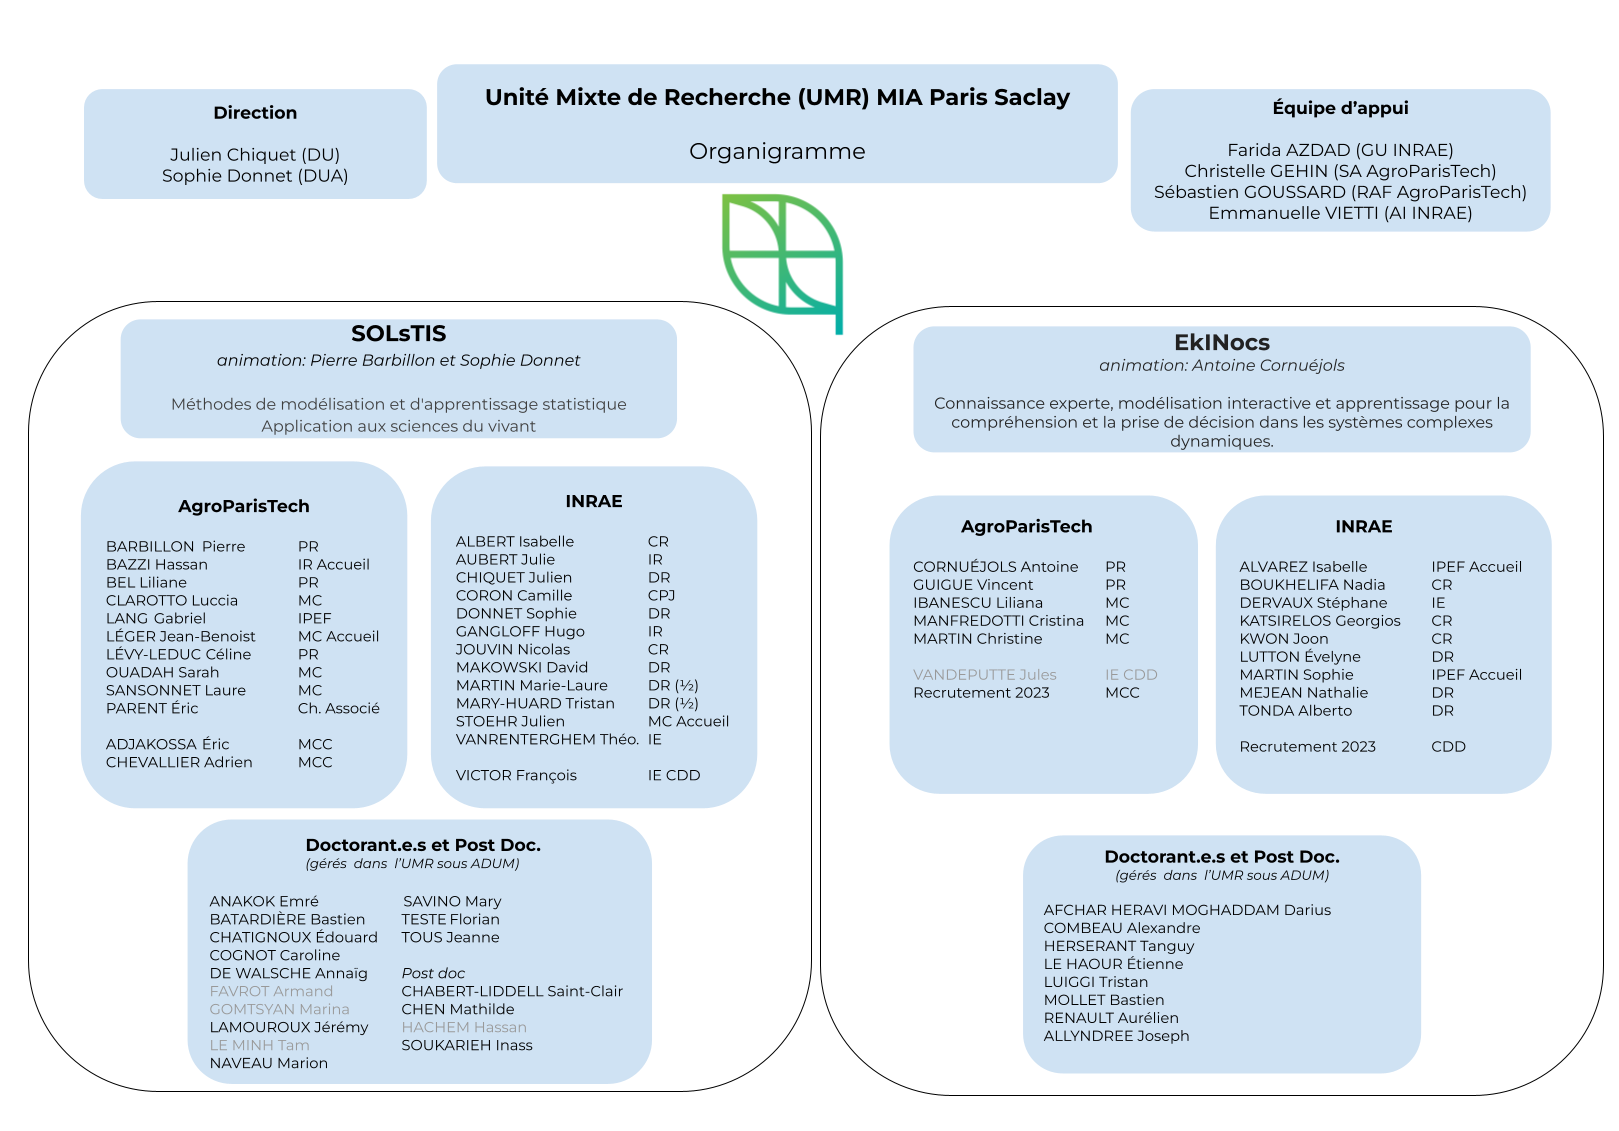
\includegraphics[width=12cm]{organigrammeEquipe.png}
        \caption{Organigramme de l'UMR MIA Paris-Saclay}\label{fig_organigrame}
        %legende
    \end{center}
\end{figure}
Les compétences mises en oeuvre portent sur les méthodes d’inférences statistiques et algorithmiques. L’unité développe des méthodes statistiques et informatiques originales, \sloppy génériques ou motivées par des problèmes précis en science du vivant. Ses activités s’appuient sur une bonne culture dans les disciplines destinatrices: écologie, environnement, agro-alimentaire, biologie moléculaire et biologie des systèmes.
L'unité MIA est dirigée par Julien CHIQUET et Sophie
DONNET, et comprends deux équipes distinctes: l'équipe SOLsTIS (Statistical
mOdeling and Learning for environnemenT and Life Science) dirigée par Sophie
DONNET et Pierre BARBILLON, et l'équipe EkiNocs (Expert Knowledge, INteractive
modelINg for understandINg and decisiOn makINg in dINamic Complexe Systems),
dirigée par Antoine CORNU\'{E}JOLS.

En tant que stagiaire, j'ai ainsi pu intégrer SOLsTIS (\cref{fig_organigrame}) pour mettre au point des
méthodes informatiques et statistiques pour l'analyse textuelle d'abstracts
d'articles scientifiques. L'unité comprends 63 membres tous statuts et équipes
confondus, dont 40 appartiennent à l'équipe SOLsTIS, 19 à l'équipe EkiNocs et 4
membres d'appui. 

\thispagestyle{fancy}

\section{Le vers de terre dans la littérature scientifique}

\noindent
Pour caractériser le rôle écologique des vers de terre d'après la littérature scientifique disponible, les abstracts (courts résumés \textbf{standardisés}) de 116 articles scientifiques issus de 4 métaanalyses distinctes ont été fournis sous forme de fichier CSV pour être analysés informatiquement. Selon la perception actuelle des spécialistes du sujet en Europe, les services écosystémiques rendus par les vers de terre sont multiples (\cref{fig_wormsservices})\cite{11_EW_benefits_summary}:

{
\renewcommand{\labelitemi}{\textbullet}
\begin{itemize}
    \item Ils permettent une meilleure aération des sols (\cite{1_aeration_sols}).
    \item Ils favorisent le recyclage des éléments nutritifs, du carbone, et du phosphore (\cite{2_recyclage_elements_nutri}).
    \item Ils jouent un rôle important dans le recyclage de la matière organique des sols (\cite{3_recyclage_matiere_orga}).
    \item Leur activité de décomposeurs (minéralisation de la matière organique) favorise la croissance d'autres organismes de l'environment, augmentant de ce fait la productivité des plantes (\cite{4_augmentation_productivite_revue}).
    \item Ils sont essentiels pour la structuration, l’entretien et la productivité des sols, forestiers, prairiaux et agricoles (\cite{5_structuration_des_sols}).
\end{itemize}
} % the "%" aims to define an environment where bullets are set to textbullet.

\noindent
Cependant, la position argumentative défendue par les spécialistes d'Amérique du Nord est très différente, pour ne pas dire radicalement opposée. On peut résumer la perception nord-américaine comme suis: 

{
\renewcommand{\labelitemi}{\textbullet}
\begin{itemize}
    \item Les vers de terre exotiques (venus d'Europe et d'Asie) sont des espèces invasives suceptibles de perturber les écosystèmes natifs (\cite{6_invasion_vers_de_terre}). Voir \cref{fig_wormmap}.
    \item Leur présence dans les sols modifie durablement les propriétés physico-chimiques des écosystèmes sousterrains (\cite{7_EW_change_soil_chemical_properties}).
    \item Les modifications physico-chimiques induites par les espèces exotiques causent une baisse globale de la biodiversité chez les espèces natives du milieu (\cite{8_EW_erode_soil_biodiversity}).
    \item L'impact de ces espèces exotiques sur les émissions de gaz à effet de serre est également sujet à controverse (\cite{9_EW_effet_serre,10_EW_pas_effet_de_serre}).
\end{itemize}
}

\begin{figure}[H] %le h entre crochet signifie je veux la figure à cet emplacement
    \begin{center} %centrer la figure
        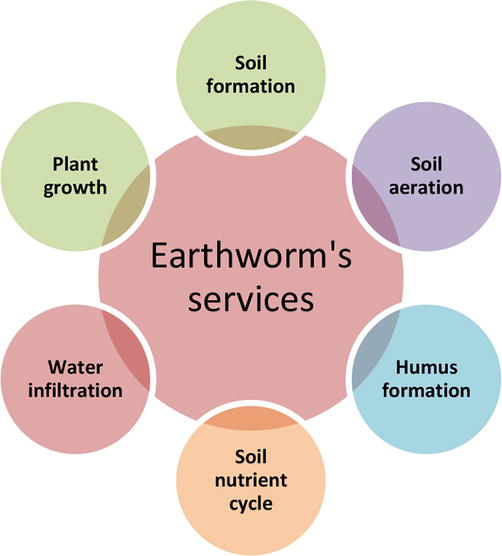
\includegraphics[width=0.2\textwidth]{EW_services.png}
        \caption{Les services écosystémiques rendus par les vers de terre.}\label{fig_wormsservices}
        %legende
    \end{center}
\end{figure}

\begin{figure}[H] %le h entre crochet signifie je veux la figure à cet emplacement
    \begin{center} %centrer la figure
        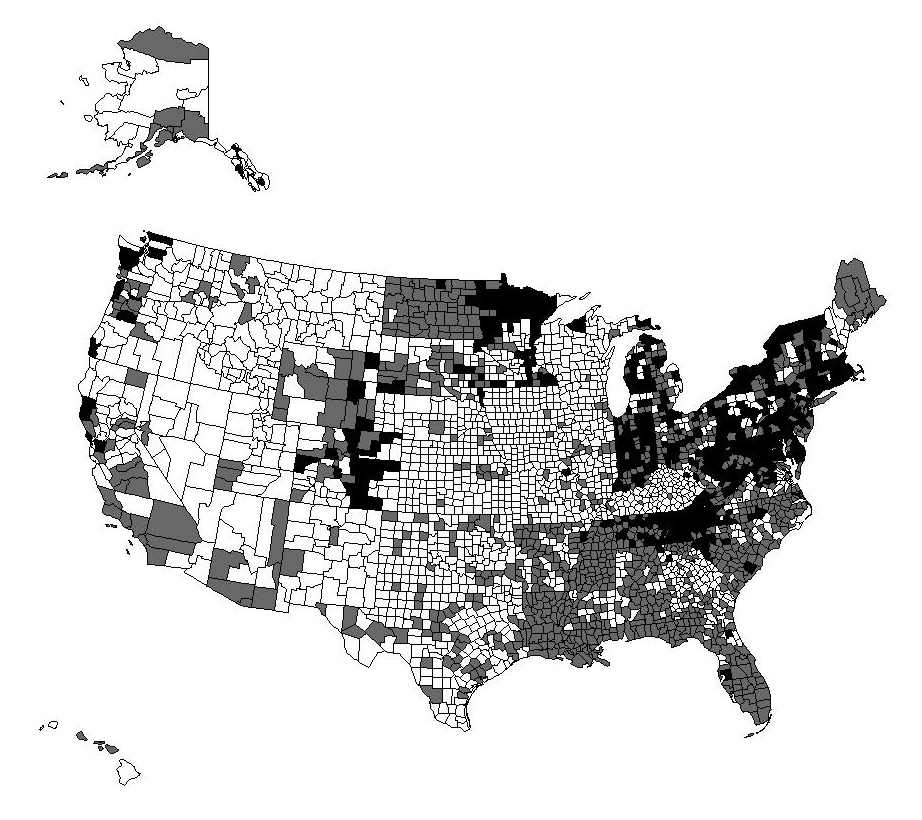
\includegraphics[width=0.3\textwidth]{worm-map.png}
        \caption[Distribution régionale de Lumbricus rubelus (espèce exotique) aux USA.]{Distribution régionale de Lumbricus rubelus (espèce exotique) aux USA. Les régions représentent les stations où: L. rubelus a été retrouvé (\textbf{noir}), une autre espèce que L. rubelus a été retrouvée (\textbf{gris}), aucune donnée n'est disponible (\textbf{blanc}).  \textit{Source:} \url{https://daphnia.ecology.uga.edu/drakelab/?p=318}.}\label{fig_wormmap}
    \end{center} 
\end{figure}

\section{Objectifs de mon travail}

\noindent
L'analyse infomatique des abstracts des articles issus des 4 métaanalyses a été conduite pour répondre à la question de recherche suivante:


\vspace{\baselineskip}
\noindent
\textbf{Les méthodes statistiques de Text-mining permettent-elles d'identifier des groupes distincts d'articles scientifiques défendant une conception opposée du rôle écologique du vers de terre au sein du corpus de texte fourni pour l'analyse?}

\vspace{\baselineskip}
Pour répondre à cette question, nous procéderons en deux étapes: 
\begin{enumerate}
    \item Création d'une base de métadonnées (comprenant notamment les \textbf{abstracts} de chaque étude indépendante formant les 4 métaanalyses) via un script Python de Web-scraping, sous forme d'un fichier CSV brut destiné à être analysé.
    \item Analyse textuelle des abstracts d'articles scientifiques présents dans le fichier CSV issu de l'étape précédante via un script R.
\end{enumerate}
\vspace{\baselineskip}
Une fois ces étapes achevées, nous discuterons les résultats obtenus et les méthodes employées en les comparant avec ceux d'autres articles de la littérature scientifique spécialisés dans ce domaine.
\thispagestyle{fancy}

\chapter[Ressources]{\label{Second Chapitre}Ressources: pratiques
  professionnelles, environnement informatique, outils informatiques et
  statistiques, données}
\section{Environnement informatique}
\noindent
Le matériel qui m'a été fourni par le laboratoire est un ordinateur fixe HP Elite SFF 800 G9 Desktop PC, numéro de série CZC2479ZXS - 4G087AV, avec 31 Go de mémoire vive et un processeur 12th Gen Intel® Core™ i7-12700 × 20, ainsi qu'un processeur graphique Mesa Intel® UHD Graphics 770. Il est géré par un système d'exploitation Ubuntu 22.04 64-bits (distribution Linux), sous la version 42.9 de GNOME (GNU Network Object Model Environment) fournissant une interface utilisateur ergonomique pour interagir avec le système d'exploitation GNU  (\textit{GNU's Not Unix}). Il est ainsi composé d'un noyeau Linux et de GNU, qui ensemble forment le système d'exploitation communément connu sous le nom "Linux". Le système de fenêtrage est "Wayland", un système chargé de l'affichage et du placement des fenêtres durant l'usage du système d'exploitation par l'utiisateur.

\section{Pratique Professionnelle}

\subsection{Veille bibliographique et technologique}
\noindent
Pour la veille bibliographique, je me suis aidé du script de Web-scraping développé dans le cadre de mon stage, qui, à partir d'un fichier comprenant les titres de nombreux articles cible, m'a permis de récupérer les métadonnées associées de maniere semi-automatique. Les journaux consultés (\textit{Applied Soil Ecology, Ecosystems, Soil Biology and Biochemistry}, etc.) étaient majoritairement orientés sur les études écologiques. Un travail par recherche MESH a aussi été réalisé, en retenant les mots-clés \textbf{Oligochaetas, Earthworm, Lumbricus terrestris, Ecosystems, Introduced species, Soil, Data mining} et \textbf{Meta-Analysis}. Pour gérer cette bibliographie, j'ai employé le package LaTeX \textit{cleveref} conçu dans ce but.

\subsection[Bonnes pratiques]{Bonne pratique de programmation informatique et
    de developpement logiciel}
\noindent
Pour l'écriture du code Python, j'ai utilisé l'éditeur de code Visual Studio Code (VScode). Pour la conception du script Rmd, j'ai travaillé sous l'IDE RStudio. Conformément aux bonnes pratiques, l'intégralité des scripts (Python et R) ont été commentés en anglais, pour faciliter la relecture du code. Pour tester le fonctionnement de chaque script, deux approches différentes ont été mises en place: 

Pour le script de Web-scraping en Python, les tests de fonctionnement effectués durant le développement ont été réalisées sur des jeux de données réduits (comprenant le plus souvent seulement les dix premiers articles) afin de pouvoir détecter rapidement si la sortie renvoyée est correcte par rapport à la tâche initiale. Pour la récupération de données via Crossref, des tests ont aussi été réalisées, notamment pour l'exploration des structures JSON renvoyées par la fonction works() de l'API. Une fois les données recherchées obtenues en sortie de tests ponctuels, il a été possible de généraliser la méthode, en l'appliquant dans l'ensemble du script principal. Enfin, afin d'éviter la régression du code (perte de fonctionnalité), j'ai souvent travaillé sur deux scripts identiques mais distincts, le premier servant de script principal, tandis que le deuxième était davantage un support pour le développement de nouvelles fonctionnalités. De cette façon, le script principal n'était mis à jour que lorsque le script secondaire était considéré comme fonctionnel. Un dépôt GitHub personnel aurait aussi pu jouer ce rôle, mais comme je travaillais seul sur cette partie, je n'en ai pas ressenti l'utlité.
    
    
Pour le script de Text-mining en Rmd sous RStudio, la plupart des tests de fonctionnement au cours du dévéloppement ont été réalisés dans la console R directement, afin d'éviter d'ajouter de nouveaux objets inutiles "test" à l'environnement R. Les processus n'ont été intégrés au script Rmd proprement dit qu'une fois leur fonctionnement testé et validé dans la console. Dans cette démarche, le fonctionnement de l'environnement R a été très utile, car cela a permis de réemployer certains objets stockés en mémoire sans avoir à les redéfinir seulement en vue d' effectuer des tests.
\subsection{Communication des travaux}
\noindent
En concertation avec mes encadrants, j'ai aussi utilisé un dépôt GitHub spécialement
mis en place pour le projet entre eux et moi, où mon travail de chaque jour a pu être sauvegardé grâce à un mécanisme de Push/Pull. De cette façon, mes encadrants ont pu facilement suivre l'évolution de mon travail et évaluer la qualité des solutions proposées. Pour faciliter l'utilisation de cet outil, le logiciel GitHub Desktop m'a été présenté, une interface utilisateur graphique facilitant grandement la visualisation et l'usage du dépôt GitHub mis en place pour le projet. Grâce à la fonctionnalité Knitr de Rmd, j'ai pu rendre compte de ma progression quotidienne en produisant automatiquement un fichier rapport au format HTML, directement issu de mon code (figures produites sous R, titres et intérprétation rédigées en Markdown ou HTML). Les réunions avec mes encadrants, le plus souvent hebdomadaires, ont été fixées par échange de mails ou bien organisées de vive voix sur site. Elles m'ont permis de rester bien focalisé sur la mission en me fournissant des objectifs hebdomadaires clairs et précis, tout en permettant à mes encadrants d'être régulièrement informés de ma progression par rapport aux objectifs fixés.

\thispagestyle{fancy}

% RECUPERER DE L'ESPACE ICI SI BESOIN EN RACOURSSISSANT LES DESCRIPTIONS.
\section[Outils informatiques et statistiques]{Outils informatiques et
  statistiques pour les différentes phases de vos travaux}
  
\subsection{Récupération des abstracts et des métadonnées avec Python}
\noindent
Pour l'élaboration du script Python, j'ai surtout utilisé le package Python Habanero Crossref pour requêter (en utilisant une API) la base de données Crossref, qui contient une grande
quantité de métadonnées (donnés sur les articles en tant que tel, comme
l'abstract, les auteurs, etc.), afin de récupérer les informations voulue à
propos d'un ensemble de titres d'articles scientifiques défini au préalable sur
le sujet des vers de terre. Pour compléter les données récupérées (la base de
Crossref comprenant de nombreuses données manquantes), j'ai aussi développé en
parallèle un module pour récupérer les données d'intérêt dans le code source de
ResearchGate (web scraping), comme le \textit{DOI (Digital Object Identifier)}
de chaque publication, la date de chargement sur la base de RG ou encore le
lien vers la page RG correspondante. Pour parvenir à cette solution, voici la liste des modules qui ont été utilisés:

\begin{description}
    \item[Pandas:] Pandas est un module qui permet de manipuler facilement des
        tableaux de données avec des étiquettes de variables (colonnes) et d'individus
        (lignes). Il est notamment utilisé dans le script pour exporter les résulats
        issus du code Python vers un fichier CSV(coma separated values), lisible et
        modifiable à l'aide d'outils de bureautique courants comme LibreOffice Calc ou
        Excel.

    \item[Numpy:] Package conçu pour le calcul scientifique avec Python. Il est
        très utile pour l'algèbre (comme par exemple pour la manipulation de matrices),
        et son implémentation en C, C++ et Fortran en fait un outil de calcul rapide et
        efficace pour l'analyse de données et le calcul scientifique. Dans le code,
        cela dit, il sert simplement à l'indexage lors de la création du DataFrame de
        résultats.

    \item[Itertools:] Module implémentant des outils Python pour maîtriser plus
        subtilement les itérations. La méthode employée dans le code est
        \textit{zip\_longest}, qui permet de créer un DataFrame à partir d'une liste de
        listes de tailles potentiellement différentes. La plus longue sera employée en
        référence (longest), et toutes les autres seront ajustées à cette longueur par
        l'ajout d'une \textit{fillvalue} ("null", dans le code). Dans mon travail, elle
        a servi à créer le DataFrame requis à partir de listes de données de tailles
        pas forcément égales (à cause des valeurs manquantes).

    \item[Habanero:] Module client de bas niveau pour interroger l'API
        Crossref, une base de données contenant les métadonnées des articles de tous les
        membres (des informations comme le titre, le nom d'auteur, le DOI etc.). Dans
        le code Python, elle est employée surtout pour rechercher les noms d'auteurs,
        les autres champs testés n'étant pas assez fiables pour automatiser
        complètement la récupération d'informations. Crossref est codé comme une
        \textbf{classe} du module Habanero, comprenant les méthodes works(), members(),
        prefixes(), funders(), journal(), type() et licence(). Dans le code Python,
        seule la méthode works() a été employée pour envoyer une requête à partir du
        titre de chaque article.

    \item[Unidecode:] Module contenant entre autres la fonction éponyme
        \textit{unidecode} (employée dans le script) conçue pour transformer les chaînes de
        caractères contenant des caractères non-ASCII (comme par exemple des
        idéogrammes chinois) pour les traduire en chaînes de caractères contenant
        uniquement des caractères ASCII. Dans le code, la fonction \textit{unidecode}
        est employée pour rendre l'affichage des noms d'auteur contenant des caractères
        non-ASCII. Certaines corrections sont imparfaites et retirent quelques lettres.

    \item[RGS2:] Sous-module codé localement à partir d'un exemple trouvé en
        ligne\footnote{citation url à mettre ici (scrape publications from RG)}
        , par la suite adapté pour récupérer directement les informations
        voulues dans le code source du site scientifique ResearchGate, les autres
        options potentielles (comme Google Scholar) ayant souvent un système de
        détection et de blocage des bots. Seule la deuxième version du sous-module a
        été retenue dans le projet final. Il dépend des modules suivants :
        
    \begin{enumerate}
        \item Module \textbf{Parsel}, fonction \textit{Selector}: Module
                facilitant l'extraction des données pour les formats HTML, JSON et XML. Dans le
                code, il est utilisé pour trouver les données recherchées directement dans le
                code source de la page (web scraping) en s'appuyant sur des sélecteurs CSS.
        \item Module \textbf{playwright.sync\_api}, fonction
                \textit{sync\_playwright}: Module permettant de lancer une session navigateur
                depuis un script Python. Dans le code, il est utilisé pour se rendre sur le
                site de ResearchGate via une session Chromium, un navigateur libre développé
                par Google.
        \item Module \textbf{re}: Module fournissant des opérations sur les
                expressions rationnelles utilisable dans un code Python. Dans le code Python, il est utilisé pour
                filtrer les résultats HTML bruts issus du Web scraping.
        \item Module \textbf{time}, fonction \textit{sleep}: Module
                fournissant différentes fonctions liées au temps. Dans le script, la fonction
                "sleep(t)" est utilisée pour forcer le système à ne rien faire pendant t
                secondes, évitant de cette façon de surcharcher le serveur cible de requêtes
                trop rapides et trop nombreuses.
    \end{enumerate}
\end{description}

\subsection{Text Mining avec R}
\noindent
Pour réaliser le text-mining, j'ai utilisé un script R (développé sous Rstudio
en Rmd) pour traiter les textes et l'analyser sous forme de figures. Mon travail a donc consisté à adapter les
codes R montrés en exemple sur des livres à mes propres données (abstracts
d'articles scientifiques), structurées différemment. Les analyses portaient par
exemple sur la fréquence des mots, au global et pour chaque MA, ou encore sur
l'analyse de sentiment reposant sur l'attribution d'un
score positif (+1) ou négatif (-1) à chaque mot du corpus. Cette attribution de
sentiment a pu être réalisée grâce à un dictionnaire R conçu pour relier un
token donné à la valence (positive ou négative) qui lui correspond. Afin de
mieux visualiser les résultats, différentes figures ont été réalisées, comme
des diagrammes en barre ou des nuages de mots. Le script R développé repose sur les librairies suivantes:

  \begin{description}
      \item[Librairie dplyr:] Librairie R conçue pour faciliter la manipulation de larges jeux de données (DataFrame et Tibble), avec des fonctions spacialisées comme \textit{mutate} (ajout de variables), \textit{select} (sélectionner les variables à partir de leurs noms), \textit{filter} (filtrer des cellules selon leur valeur), \textit{summarise} (résumer les informations d'un tibble dans un format très synthétique) et \textit{arrange} (pour réordonner les lignes selon l'ordre / la variable voulue.)
      \item[Librairie ggplot2:] Librairie R pour créer déclarativement des graphiques divers et variés (barplots, histogrammes, scatter plots, etc.)
      \item[Librairie tidytext:] Librairie R conçue pour faciliter l'analyse de texte (Silge, Julia, and David Robinson. 2016. "tidytext: Text Mining and Analysis Using Tidy Data Principles in R."\footnote{ref Silge/Robinson à mettre à la place}), se fondant sur le paradigme d'analyse de données "tidy", où chaque variable est une colonne, chaque observation une ligne et chaque ensemble d'observations est un tableau. La fonction la plus utilisée dans le cadre de cette analyse est \textit{unnest\_tokens}, qui permet de transformer un texte donné en une tables d'unités textuelles plus réduites (tokens), comme des phrases ou des mots.
      \item[Librairie Knitr:] Librairie R conçue pour récupérer automatiquement l'output d'un code R (par exemple, pour produire une figure) afin de l'inclure dans un autre document (par exemple, format Word, HTML ou PDF) qui contiendra aussi la prose écrite par l'auteur du document, souvent pour interpréter ou commenter des résultats. Cette librairie permet notamment de moduler plus finement l'affichage des résultats, en permettant par exemple de ne pas afficher certaines figures dans un format de sortie donné (pour masquer une figure interactive au format HTML que l'on ne souhaite pas forcément voir apparaître dans un document PDF, par exemple).
      \item[Librairie SnowballC:] Librairie R implémentant Snowball, un langage conçu pour gérer les chaînes de caractères, les nombres entiers et les booléens. Dans le script R de Text Mining, il a servi à transformer les tokens pour ne garder que la racine de chaque mot (processus de \textit{racination}), afin d'éviter les erreurs de comptage (si, pour un humain, "enhance" et "enhancement" sont deux mots ayant approximativement le même sens, informatiquement ce sont deux chaînes de caractères distinctes).
      \item[Librairie grid:] Librarie R implémentant les fonctions graphiques primitives\sloppy qui sous-tendent le package ggplot2. Elles permettent de modifier certains détails des graphes produits grâce à ggplot2, offrant ainsi un meilleur contrôle du rendu visuel du résulat obtenu. Dans le script, il est employé, par exemple, pour spécifier exactement l'aspect des flèches composant le réseau de bigrammes. 
      \item[Librairie ggraph:] Librairie R formant une extension de ggplot2, conçue pour permettre de supporter les structures de données relationnelles comme les réseaux, les graphes et les arbres. Dans le script, elle est notamment employée pour produire les réseaux de bigrammes.
      \item[Librairie igraph:] fonction \textit{graph\_from\_data\_frame():} Cette fonction appartient à la librairie igraph. Elle crée un objet graphe à partir d'un data frame, où le data frame représente les arêtes entre les nœuds.
      \item[Librairie egg:] fonction \textit{ggarrange():} Librairie servant à organiser différents graphes sur une seule et même figure. Dans le script, c'est l'une des librairies employées pour comparer les quatre MA entre elles.
      \item[Librairie tidyr:] Librairie R implémentant des méthodes utiles pour manipuler des objets de type "tidy". Elle comprend des fonction telles que \textit{pivot\_wider} et \textit{pivot\_longer} (pour convertir le dataFrame d'un format à un autre), ou encore \textit{bind\_rows()}, pour combiner des DataFrames par lignes.
  \end{description}

\section{Données}
\noindent
L'approche "tidy" choisie repose sur la \textit{tokenisation} du corpus
de texte en unitées textuelles (appelées \textit{"tokens"}) plus petites, comme
des mots, des phrases ou des \textit{n-grams}. J'ai pour cela pu m'inspirer du
livre rédigé par Julia Slige (data scientist) et David Robinson (Directeur de
Data Scientist de la plateforme Heap). \footnote{disponible en ligne à l'adresse:
https://www.tidytextmining.com/.} Afin de filtrer les mots d'intérêt seulement, deux stratégies ont été
employées: Premièrement, un filtrage brut de tous les mots de liaisons sans
rapport direct avec le sujet (nommés "stop words" en text-mining, des mots tels
que "the", "and", "is", "of" etc. en anglais) pour ne conserver que les mots
sur lesquels les analyses pourront donner des résultats scientifiques
significatifs (savoir que le mot "le" est le plus fréquent dans un corpus de
texte français ne signifie rien sur le plan biologique). Deuxièmement, une
autre approche a été de considérer la fréquence de chaque mot par rapport au
nombre total de mots présents dans le corpus (n mot / N mots). De cette façon,
les mots les plus fréquents perdent une partie de leur poids statistique, tandis que les mots plus rares en gagnent. On peut ainsi visualiser facilement les mots les plus importants d'un texte, sans même
avoir besoin de modifier les données au préalable avec une liste de stop words.
Cela permet de conserver le texte dans son ensemble, évitant ainsi un potentiel
biais pouvant perturber l'analyse.

\chapter{\label{Troisième Chapitre}Résultats}
\section{Web-scraping et obtention d'une base de métadonnées en format CSV}
\noindent
En sortie du code de Web-scraping dévéloppé en Python (et après recherche manuelle des données manquantes), un fichier de métadonnées au format CSV, contenant la métaanalyse d'origine, le titre, les auteurs, l'abstract, la date de publication sur ResearchGate, le DOI et l'URL vers la page RG correspondante a été obtenue (\cref{fig_CSV}). 

\begin{figure}[H] %le h entre crochet signifie je veux la figure à cet emplacement
    \begin{center} %centrer la figure
        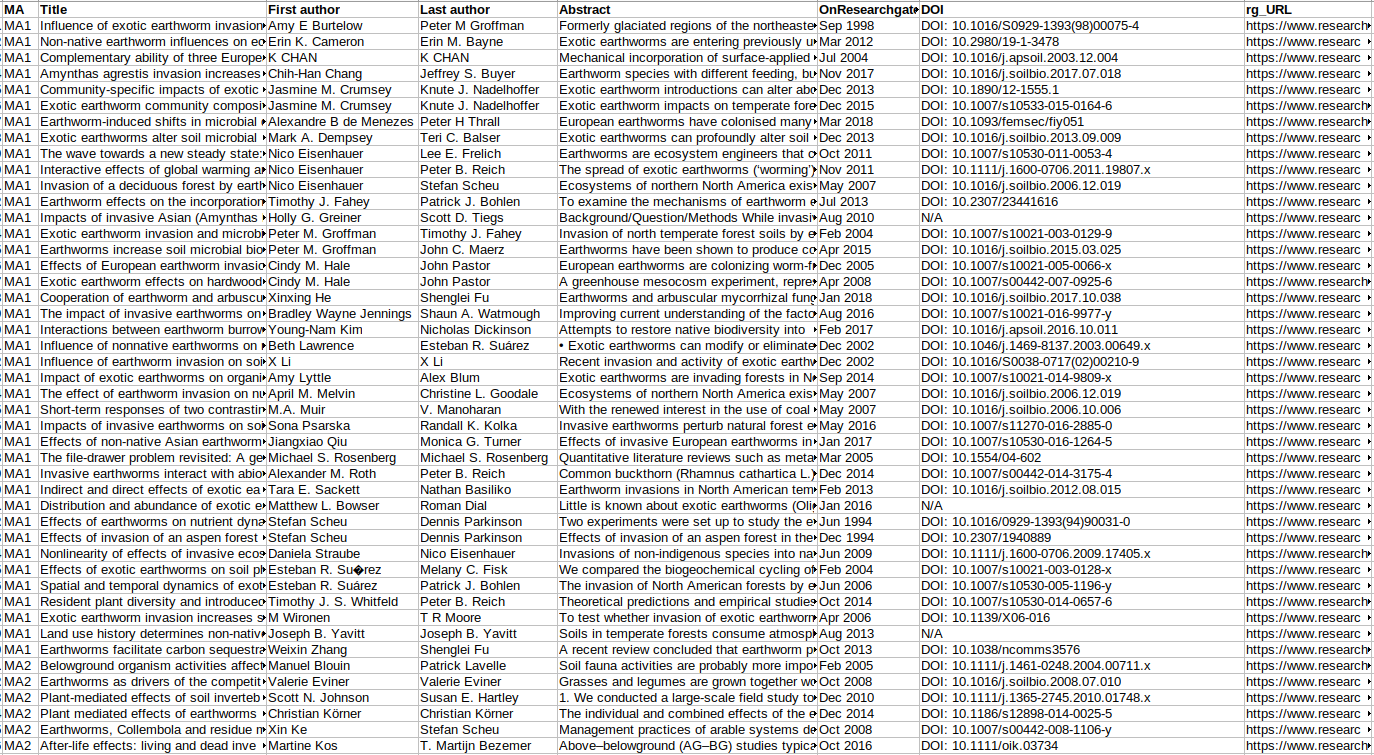
\includegraphics[width=1.1\textwidth]{exemple_CSV_rogne2.png}
        \caption{Impression écran montrant les 46 premières lignes du fichier CSV issu du Web-scraping et employé comme base de données pour la suite des analyses. Les données manquantes restante après complétion manuelle sont représentées par "N/A". Malgré l'usage de la fonction Python "unidecode" (voir Chapitre 2.3.1), certains caractères spéciaux ne sont toujours pas reconnus et sont notés
\includegraphics[width=0.03\textwidth]{diamond-question-mark.jpeg}.}\label{fig_CSV}
        %legende
    \end{center}  
\end{figure}

\section{Analyse globale des textes bruts}
\noindent
Pour détecter informatiquement les racines les plus fréquentes du corpus, chaque token distinct (dans cette section, des mots uniques) présent dans les quatre jeux de données (abstracts d'articles) a été compté.  Le graphique ci-dessous présente les racines les plus fréquemment retrouvées dans l'ensemble du corpus. Les trois plus imporantes sont \textbf{earthworm}, \textbf{soil} et \textbf{plant} (\cref{freq_all}).

\begin{figure}[H] %le h entre crochet signifie je veux la figure à cet emplacement
    \begin{center} %centrer la figure
        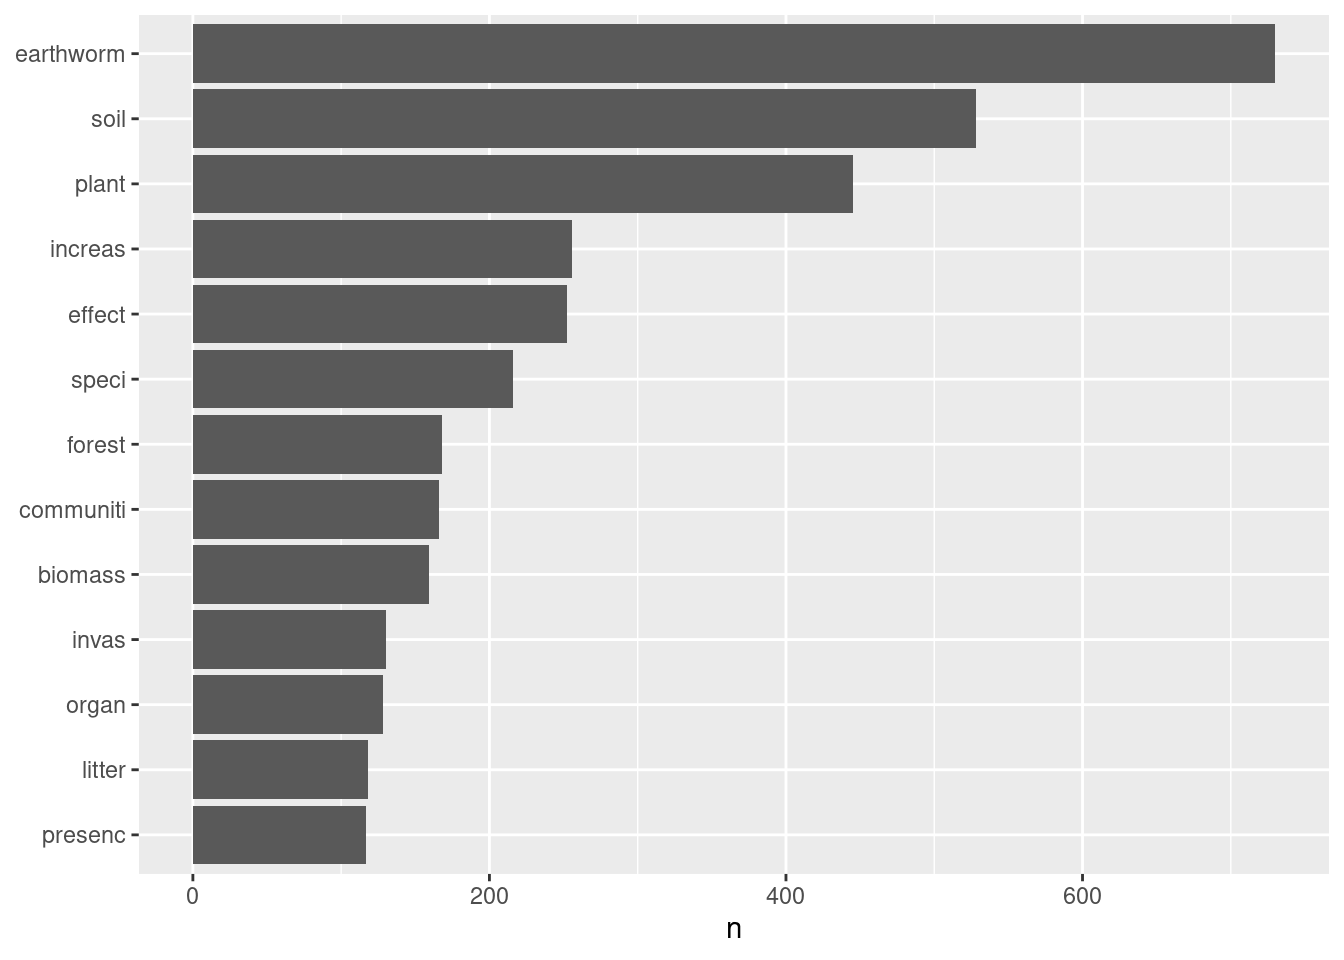
\includegraphics[width=1\textwidth]{freq_all_MA.png}
        \caption{Sur l'axe des abscisses, les valeurs numériques représentent le nombre total d'occurences des mots (après \textit{racination}) écrits en ordonnées. On remarque que les trois mots les plus fréquents dans les articles des quatres métaanalyses confondues sont \textbf{earthworm}, \textbf{soil} et \textbf{plant}.\label{freq_all}}
        %legende
    \end{center}  
\end{figure}

Dans un second temps, on a conduit la même analyse, mais en considérant cette fois-ci chaque métaanalyse comme un sous jeu de données à part entière (\cref{freq_each}). Les résultats observés pour chaque métaanalyse sont différents des résulats globaux, avec \textbf{earthworm}, \textbf{soil} et \textbf{forest} en premier pour la MA1, \textbf{plant}, \textbf{earthworm} et \textbf{increase} pour la MA2, \textbf{earthworm}, \textbf{species} et \textbf{plant} pour la MA3 et \textbf{earthworm}, \textbf{plant} et \textbf{soil} pour la MA4. Si tous ces groupes ne sont certes pas identiques, on remarque la prévalence de "earthworm" et de "plant", ainsi que la mention de certains écosystèmes ("soil", "forest"). La racine "invas" est aussi présente dans les graphes de fréquence des MA1 et 3.

% Pour des raisons de taille de cette section et de complexité d'interprétation, le scale graph n'a pas été inclus ici. Sélection à discuter.

\begin{figure}[H] %le h entre crochet signifie je veux la figure à cet emplacement
    \begin{center} %centrer la figure
        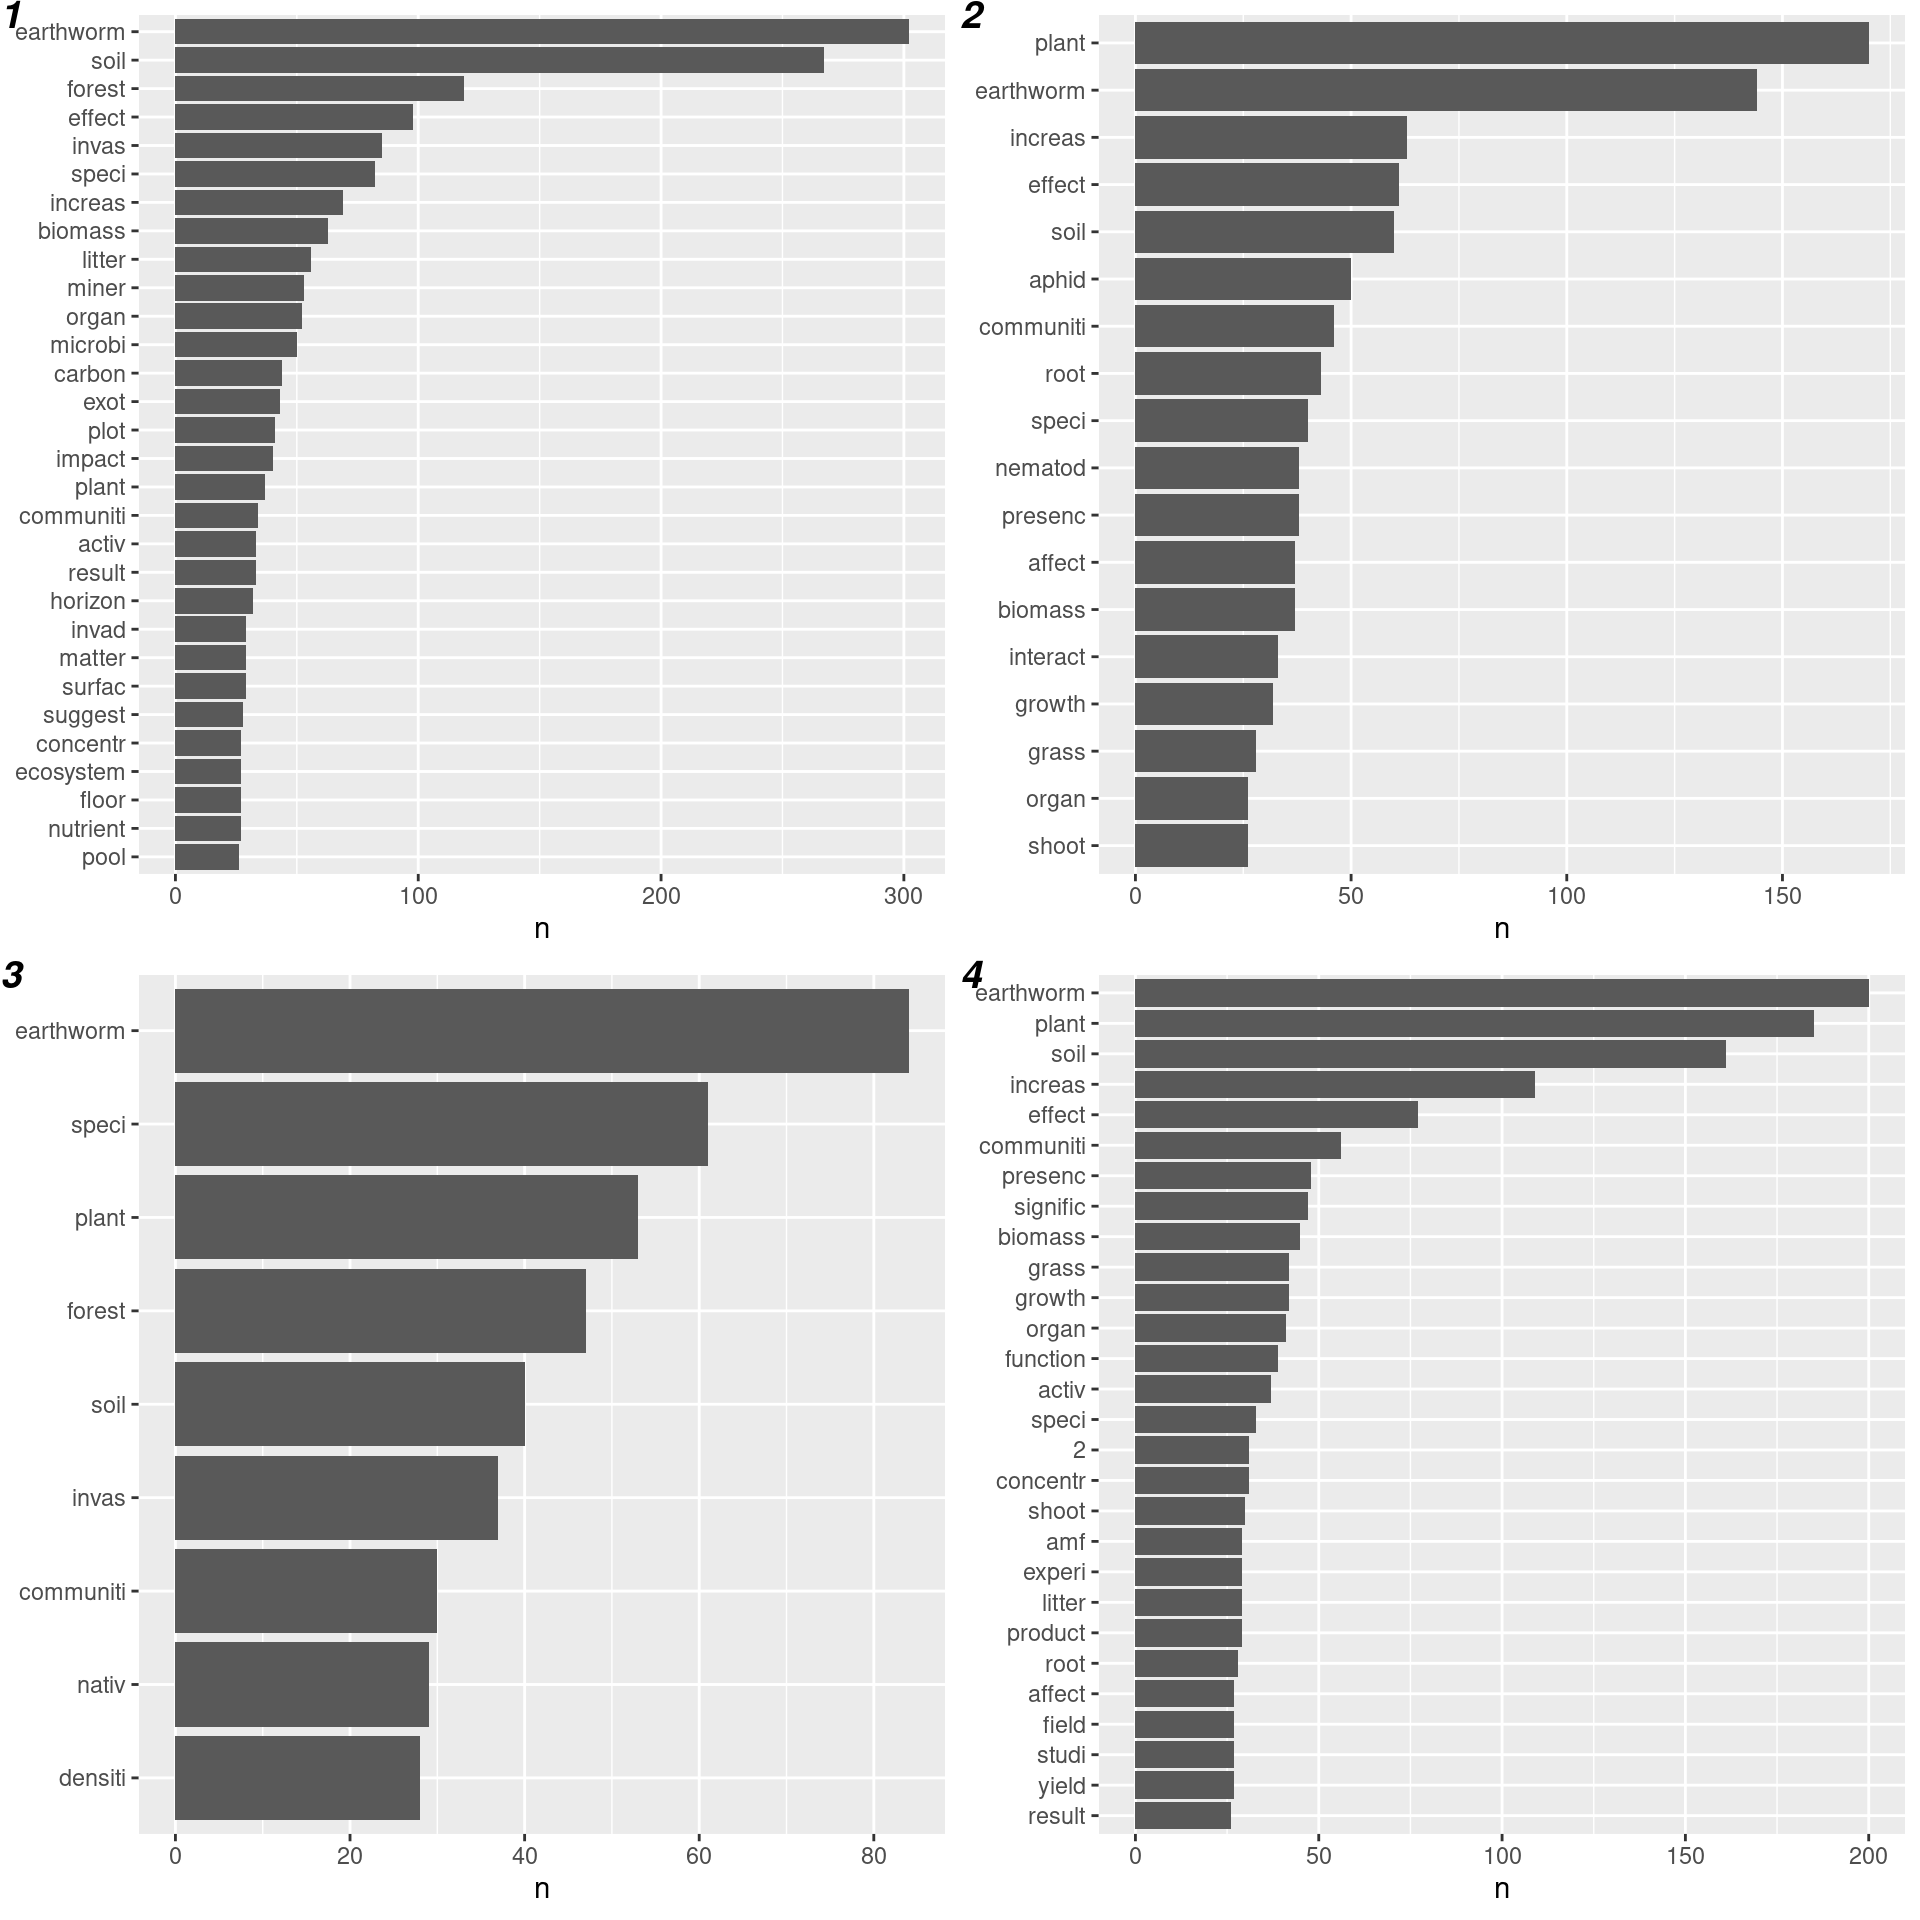
\includegraphics[width=1\textwidth]{freq_each_MA.png}
        \caption{Sur l'axe des abscisses, les valeurs numériques représentent le nombre total d'occurences des mots (après \textit{racination}) écrits en ordonnées. On remarque que les résultats individuels sont très différents de ceux obtenus lors de l'analyse collective.\label{freq_each}}
        %legende
    \end{center}  
\end{figure}

\section{Analyse de sentiment}
\noindent
L'objectif de cette série d'analyses est de détecter informatiquement l'avis émis par les abstracts composant le corpus de texte à propos de leur sujet d'étude (ici, les vers de terre). Pour cela, on s'appuie sur des dictionnaires R prédéfinis faisant correspondre à chaque mot un score chiffré, +1 si le mot est positif, -1 sinon. La visualisation sous forme de nuage de mots (\cref{senti_cloud_all}) permet de constater que les racines "invasiv", "invad" et "effect", "affect" ont été les plus importantes contributrices au score de sentiment global.

\begin{figure}[H] %le h entre crochet signifie je veux la figure à cet emplacement
    \begin{center} %centrer la figure
        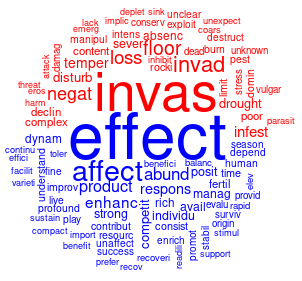
\includegraphics[width=0.5\textwidth]{senti_cloud_all.png}
        \caption{Nuage de mots de l'ensemble des racines de mots trouvées dans la base de données. Les mots exprimant un sentiment négatif sont en \textbf{rouge}, les mots exprimant un sentiment positif en \textbf{bleu}.\label{senti_cloud_all}}
        %legende
    \end{center}  
\end{figure}

Afin de visualiser plus précisément quels mots ont été les principaux contributeurs au score de sentiment pour les quatre métaanalyses, une analyse plus détaillée a pu être mise en place pour chacune (\cref{senti_contri_each}). On peut voir que les métaanalyses 1 et 3 semblent globalement négatives (encadrés 1 et 3), tandis que les métaanalyses 2 et 4 semblent globalement positives (encadrés 2 et 4). Le nombre de contributeurs défferents est visible en ordonnée. 

\begin{figure}[H] %le h entre crochet signifie je veux la figure à cet emplacement
    \begin{center} %centrer la figure
        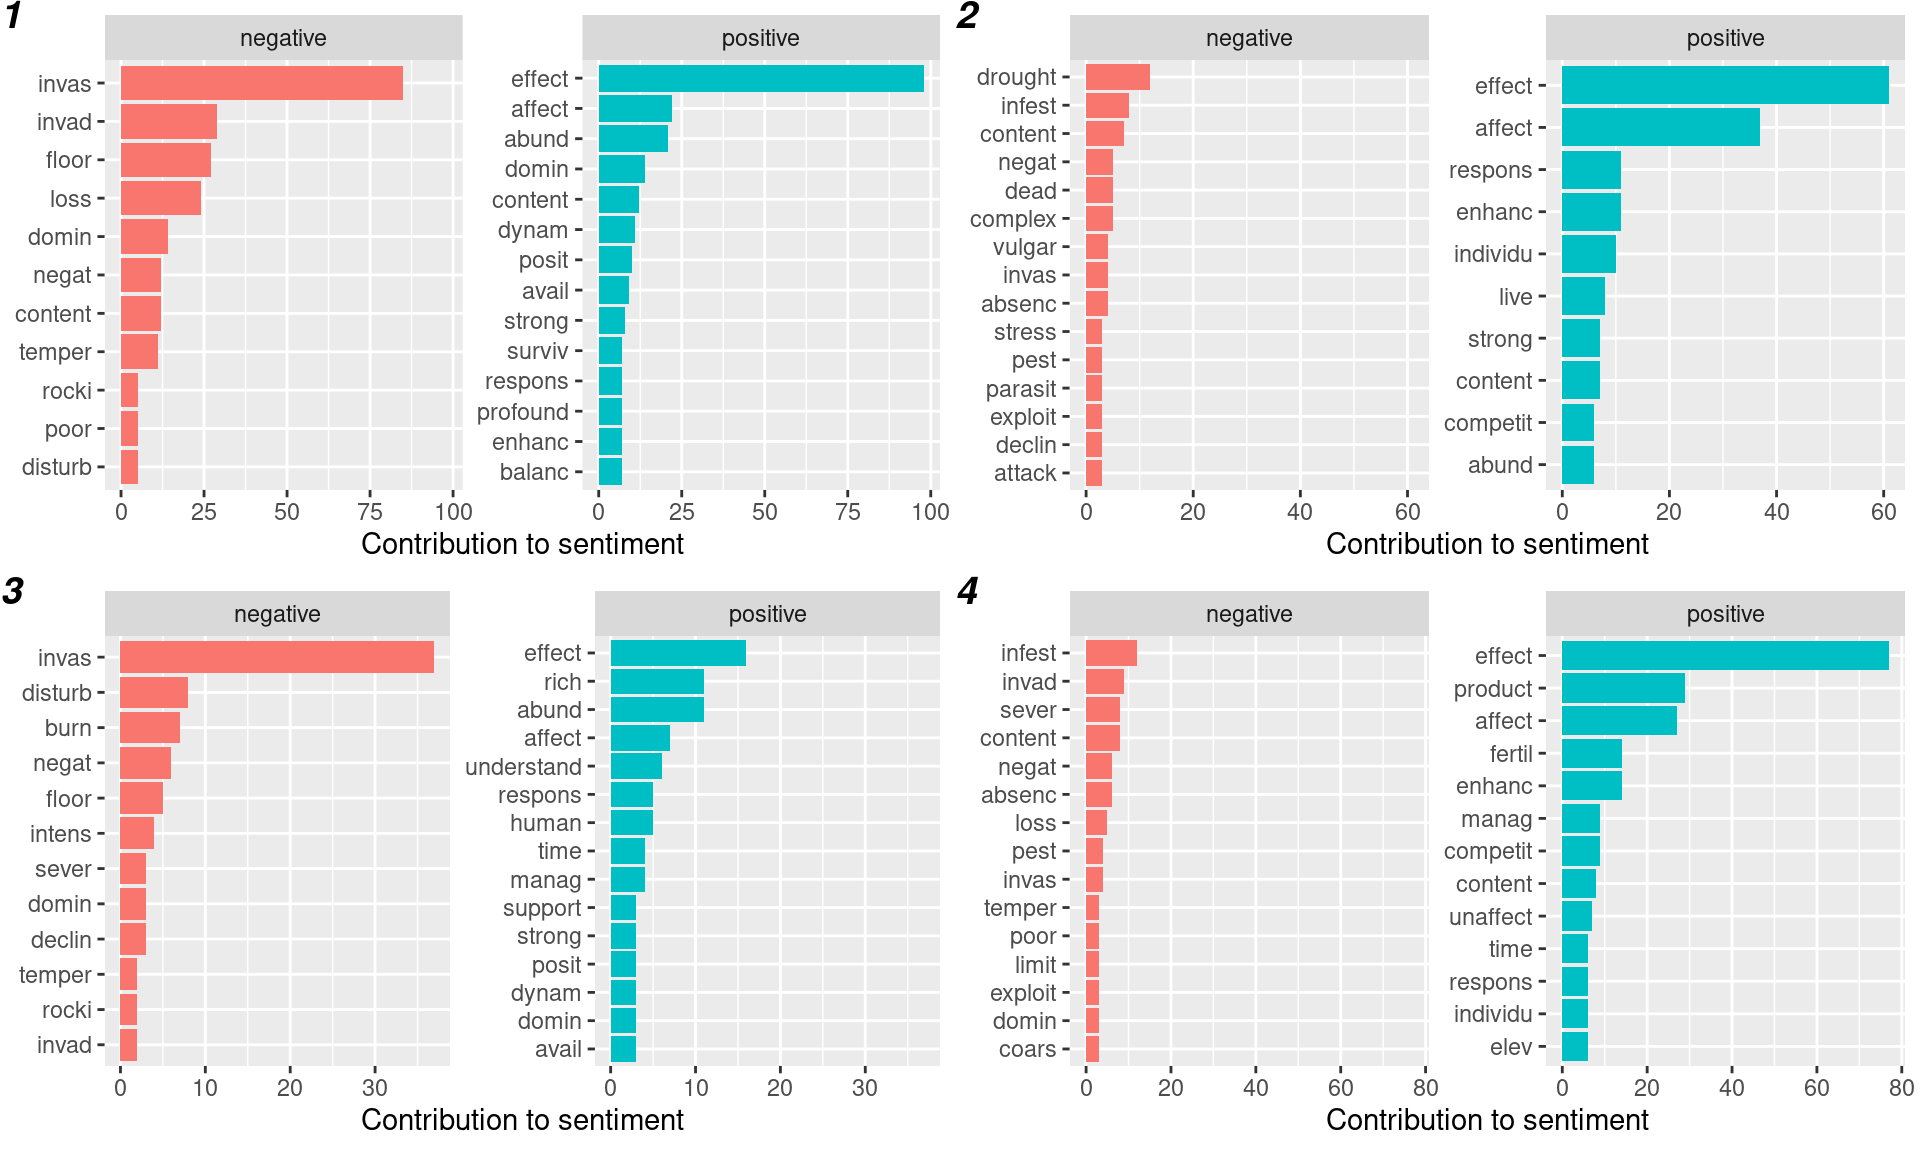
\includegraphics[width=0.9\textwidth]{senti_contri_each.png}
        \caption{Mots contribuant au score de sentiment pour chacune des quatre métaanalyses. Les mots exprimant un sentiment négatif sont en \textbf{rouge}, les mots exprimant un sentiment positif en \textbf{bleu}. Le nombre de contributeurs différents est visible sur l'axe Oy de chaque graphique.\label{senti_contri_each}}
        %legende
    \end{center}  
\end{figure}


\section{Approche tf-idf et loi de Zipf}
\noindent
L'objectif de l'approche tf-idf est d'évaluer l'importance d'un terme contenu dans un document, relativement à l'ensemble du corpus. La fréquence brute du terme est nommée tf, et la fréquence inverse de document (une mesure de l'importance du terme dans l'ensemble du corpus) est nommée idf. Le poids ajusté de chaque terme s'obtient en multipliant ces deux mesures, et il augmente proportionnellement au nombre d'occurrences du mot dans le document.

\section{Analyses de bigrammes seuls}

\section{Réseaux de bigrammes}

\thispagestyle{fancy}

\chapter{\label{Quatrième Chapitre}Discussion}
%\paragraph{Paragraphe}
\noindent
Au cours de ce stage, j'ai commencé par développer un programme Python pour le
web scraping sur la base de données médicale PubMed, avant de découvrir que ce
n'était pas selon dont nous avions besoin. J'ai donc réussi à m'adapter pour
faire fonctionner mon code (en interrogeant une autre base de données), mais il
reste encore à nettoyer les données extraites par le code (collectées
directement en brut dans un fichier CSV généré par le script).
Rétrospectivement, je ne suis pas certain que cette approche automatisée soit
vraiment rentable en temps, même si je suis satisfait d'avoir commencé à
apprendre comment développer ce type d'approches automatisées.

\lipsum[1]

\thispagestyle{fancy}

\chapter{\label{Cinquième Chapitre}Conclusion}
Elle vise, à reformuler les objectifs visés, énoncer les résultats essentiels
obtenus, à replacer le
travail dans son contexte scientifique et à faire ressortir leur importance
théorique, pratique, tech-
nique ou économique. Elle peut ouvrir de nouvelles perspectives ou hypothèses
qui seront le point
de départ de nouveaux travaux. Il n'y a pas a priori d'appel à des références.

\thispagestyle{fancy}

%%%%%%%%%%%%%%%%%%%%%%%%%%%%%%%%%%%%%%%%          15         %%%%%%%%%%%%%%%%%%%%%%%%%%%%%%%%%%%%%%%%%%%%%%%%%%%%%%%%%%%%%%%%%%%%%%%%%%%%%%%%%%%%%%%%%% Références %%%%%%%%%%%%%%%%%%%%%%%%%%%%%%%%%%%%%%%%%%%%%%%%
\newpage
\bibliographystyle{plain}
\bibliography{biblio.bib}
\thispagestyle{fancy}
%\apalike

%%%%%%%%%%%%%%%%%%%%%%%%%%%%%%%%%%%%%%%%          16            %%%%%%%%%%%%%%%%%%%%%%%%%%%%%%%%%%%%%%%%%%%%%%%%%%%%%%%%%%%%%%%%%%%%%%%%%%%%%%%%%%%%%%%%%% Verso Résumé %%%%%%%%%%%%%%%%%%%%%%%%%%%%%%%%%%%%%%%%%%%%%%%%

\newpage
\thispagestyle{empty}
\mbox{} % Insère une boîte vide

%%%%%%%%%%%%%%%%%%%%%%%%%%%%%%%%%%%%%%%%          17            %%%%%%%%%%%%%%%%%%%%%%%%%%%%%%%%%%%%%%%%%%%%%%%%%%%%%%%%%%%%%%%%%%%%%%%%%%%%%%%%%%%%%%%%%% Résumé %%%%%%%%%%%%%%%%%%%%%%%%%%%%%%%%%%%%%%%%%%%%%%%%

\newpage
\thispagestyle{empty}
\begin{center}
    \huge{\textbf{Résumé}}
\end{center}

\vspace{1cm}
à faire à la fin
\vspace{\baselineskip} % Sauter une ligne
\par
\textbf{Mots-clés de référencement type MESH:} Lumbricus terrestris, Soil, Ecosystem, Introduced species, Meta-Analysis.
\vspace{\baselineskip} % Sauter une ligne
\par
\textbf{Mots-clés des acquis techniques:} Web-scraping, Text-mining, dplyr, R Markdown, GitHub.

\end{document}

%\it = italique
% \sl = mettre en travers
% {\bf texte}
%\textbf{texte}
%vfill
%hspace{2cm} va mettre un espace entre les logos
% \thispagestyle{empty}
% renewcommand{\thechapter{Roman}} = redefinir la maniere dont la numerotation se fait pour les chaptire :refaire la commande en chiffre romain
% renewcommand{\thechapter{roman}} = chiffres romains en minuscules
% renewcommand{\thechapter{Arabic}}
%\arabic % à mettre avant le begin du doc
%\alph
%créer une nouvelle commande : \newcommand{\convertToBW}[1]{\adjustimage{filter=gray}{#1}}
%le _ permet de mettre en indice. Il peut facilement tout bousiller si mal utilisé.
% (\href{https://www.reddit.com/r/Python/comments/v2bxyl/script_scraping_researchgate_all_publications/}{\texttt{https://www.redd\linebreak it.com/r/Python/comments/v2bxyl/script\_scraping\_researchgate\_all\_publica\linebreak tions/}})


